% DPF 09 talk on strangeness in nucleon

\documentclass[10pt]{beamer}
\usepackage{amsmath}
\usepackage{mathtools}
%\documentclass[12pt]{beamerthemeSam.sty}
\usepackage{epsf}
%\usepackage{pstricks}
%\usepackage[orientation=portrait,size=A4]{beamerposter}
\geometry{paperwidth=160mm,paperheight=120mm}
%DT favorite definitions
\def\LL{\left\langle}	% left angle bracket
\def\RR{\right\rangle}	% right angle bracket
\def\LP{\left(}		% left parenthesis
\def\RP{\right)}	% right parenthesis
\def\LB{\left\{}	% left curly bracket
\def\RB{\right\}}	% right curly bracket
\def\PAR#1#2{ {{\partial #1}\over{\partial #2}} }
\def\PARTWO#1#2{ {{\partial^2 #1}\over{\partial #2}^2} }
\def\PARTWOMIX#1#2#3{ {{\partial^2 #1}\over{\partial #2 \partial #3}} }

\def\rightpartial{{\overrightarrow\partial}}
\def\leftpartial{{\overleftarrow\partial}}
\def\diffpartial{\buildrel\leftrightarrow\over\partial}

\def\BI{\begin{itemize}}
\def\EI{\end{itemize}}
\def\BE{\begin{displaymath}}
\def\EE{\end{displaymath}}
\def\BEA{\begin{eqnarray*}}
\def\EEA{\end{eqnarray*}}
\def\BNEA{\begin{eqnarray}}
\def\ENEA{\end{eqnarray}}
\def\EL{\nonumber\\}


\newcommand{\map}[1]{\frame{\frametitle{\textbf{Course map}}
\centerline{\includegraphics[height=0.86\paperheight]{../../map/#1.png}}}}
\newcommand{\wmap}[1]{\frame{\frametitle{\textbf{Course map}}
\centerline{\includegraphics[width=0.96\paperwidth]{../../map/#1.png}}}}

\newcommand{\etal}{{\it et al.}}
\newcommand{\gbeta}{6/g^2}
\newcommand{\la}[1]{\label{#1}}
\newcommand{\ie}{{\em i.e.\ }}
\newcommand{\eg}{{\em e.\,g.\ }}
\newcommand{\cf}{cf.\ }
\newcommand{\etc}{etc.\ }
\newcommand{\atantwo}{{\rm atan2}}
\newcommand{\Tr}{{\rm Tr}}
\newcommand{\dt}{\Delta t}
\newcommand{\op}{{\cal O}}
\newcommand{\msbar}{{\overline{\rm MS}}}
\def\chpt{\raise0.4ex\hbox{$\chi$}PT}
\def\schpt{S\raise0.4ex\hbox{$\chi$}PT}
\def\MeV{{\rm Me\!V}}
\def\GeV{{\rm Ge\!V}}

%AB: my color definitions
%\definecolor{mygarnet}{rgb}{0.445,0.184,0.215}
%\definecolor{mygold}{rgb}{0.848,0.848,0.098}
%\definecolor{myg2g}{rgb}{0.647,0.316,0.157}
\definecolor{abtitlecolor}{rgb}{0.0,0.255,0.494}
\definecolor{absecondarycolor}{rgb}{0.0,0.416,0.804}
\definecolor{abprimarycolor}{rgb}{1.0,0.686,0.0}
\definecolor{Red}           {cmyk}{0,1,1,0}
\definecolor{Grey}           {cmyk}{.7,.7,.7,0}
\definecolor{Lg}           {cmyk}{.4,.4,.4,0}
\definecolor{Blue}          {cmyk}{1,1,0,0}
\definecolor{Green}         {cmyk}{1,0,1,0}
\definecolor{Brown}         {cmyk}{0,0.81,1,0.60}
\definecolor{Black}         {cmyk}{0,0,0,1}

\usetheme{Madrid}


%AB: redefinition of beamer colors
%\setbeamercolor{palette tertiary}{fg=white,bg=mygarnet}
%\setbeamercolor{palette secondary}{fg=white,bg=myg2g}
%\setbeamercolor{palette primary}{fg=black,bg=mygold}
\setbeamercolor{title}{fg=abtitlecolor}
\setbeamercolor{frametitle}{fg=abtitlecolor}
\setbeamercolor{palette tertiary}{fg=white,bg=abtitlecolor}
\setbeamercolor{palette secondary}{fg=white,bg=absecondarycolor}
\setbeamercolor{palette primary}{fg=black,bg=abprimarycolor}
\setbeamercolor{structure}{fg=abtitlecolor}

\setbeamerfont{section in toc}{series=\bfseries}

%AB: remove navigation icons
\beamertemplatenavigationsymbolsempty
\title[Work and potential energy -- problem solving]{
  \textbf {Energy methods -- problem solving}\\
%\centerline{}
%\centering
%\vspace{-0.0in}
%\includegraphics[width=0.3\textwidth]{propvalues_0093.pdf}
%\vspace{-0.3in}\\
%\label{intrograph}
}

\author[W. Freeman] {Physics 211\\Syracuse University, Physics 211 Spring 2015\\Walter Freeman}

\date{\today}

\begin{document}

\frame{\titlepage}

\frame{\frametitle{\textbf{Announcements}}
\BI
\item{Mastering Physics due Monday}
\item{If your exam was misgraded, grade appeals will be handled the same way as before (and faster!)}
\EI
}

\frame{\frametitle{\textbf{Where we've been, where we're going}}
  \BI
  \large
\item{Last time: we saw that ``potential energy'' is both a statement about nature and a bookkeeping trick to keep track of work}
\BI
\item{Potential energy only applies to conservative forces (gravity, springs)}
\item{Lets us account for the work done by these forces with no integrals required}
\item{Potential energy due to Earth's gravity: $U_g = mgy$}
\item{Potential energy due to universal gravity: $U_G = -\frac{GMm}{r}$}
\item{Potential energy in a spring: $U_e = \frac{1}{2}k(\Delta x)^2$}
  \EI
\item{This time: we'll introduce the idea of {\bf power}, a rate of doing work}
  \pause
\item{... then we'll spend most of today just doing practice problems.}
  \EI
}

\frame{\frametitle{\textbf{Power}}
\large
\BI
\item{We've been concerned with quite a few ``rates`` in this class:}
  \BI
\item{Velocity: the rate of changing position, measured in meters per second}
\item{Angular velocity: the rate of changing angle, measured in radians per second}
\EI
\item{What about the rate of transfer of energy? What units would it be measured in?}
\pause
\item{This quantity is called {\bf power}}
\item{It's measured in joules per second: 1 J/s = 1 watt}
  \EI
}

\frame{\frametitle{\textbf{Power: applications}}
  \large
  When does this idea of a rate of transferring energy or doing work come up?

  \bigskip
  \bigskip
  
  \BI
\item{Rates of energy transfer: ``Sunlight delivers about 1000 watts per square meter to the ground''}
\item{Rates of energy ``consumption'': ``My laptop uses about 20 watts of power''}
\item{Rates of doing work: ``This car's engine can put out 75 kW of power''}
\EI
  
\bigskip
  \bigskip

Most of our ideas here are stepping stones to understanding something else.

The idea of power is more of a standalone concept: a useful application.

Many of our machines are limited by the {\bf rate} that they can convert energy from one form to another.
}

\frame{\frametitle{\textbf{Power: rate of doing work}}
\large
A bit of mathematics that will be useful to you:

\bigskip

{\bf ``An object moves at a constant speed $\vec v$, subject to some force $\vec F$; at what rate does that force do work on the object?''}

\bigskip

An example: an airplane flies at v=1000 m/s, and its engines exert F=300 kN of thrust. What is the rate at which the engines do work (power)?

\bigskip

\centerline{Work = force $\times$ distance}
\pause
\centerline{Power = work / time}
\pause
\centerline{Power = force $\times$ distance / time}
\pause
\centerline{Power = force $\times$ (distance / time)}
\pause
\centerline{Power = force $\times$ velocity}
\pause
\centerline{$P = \vec F \cdot \vec v = {\color{Red}300 MW}$}

\bigskip

\BI
\item{The engines output 300 MW of power: this is around 10 liters per second of fuel even at 100\% efficiency!}
  \item{Some of that 300 MW of energy dissipated by drag heats up the airplane...}
    \EI
  }

  \frame{\frametitle{\textbf{Sample problems}}
    \Large
  A truck pulling a heavy load with mass $m=4000$ kg wants to drive up a hill at a $30^o$ grade.

  \bigskip
  \bigskip

  If the truck's engine can produce 100 kW of power (134 hp), how fast can the truck go? (Neglect drag.)

}

\frame{\frametitle{\textbf{Sample problems}}
    \Large
A 1000 kg car has an engine that produces up to P=100 kW of power. If it accelerates as hard as it can, at what speed
does its acceleration become limited by the engine? 

\bigskip
\bigskip
\pause

(What else would limit its acceleration?)

\bigskip
\bigskip
\pause

At low speeds: static friction limits acceleration\\
At high speeds: engine power limits acceleration}


\frame{\frametitle{\textbf{Sample problems}}
    \Large
  If I want to shoot a bullet up from the Earth and have it fly out forever, what must its velocity be?
\pause

\bigskip
\bigskip

\centerline{$\frac{1}{2}mv_0^2 + U_{G,0} = \frac{1}{2}mv_f^2$}
\bigskip
\centerline{$\frac{1}{2}mv_0^2 - \frac{GMm}{r} = 0$}
\bigskip
\centerline{$v_0 = \sqrt{\frac{2GM}{r}} = 11.2$ km/s (``escape velocity'')}

\pause

\centerline{How can I ``cheat'' here?}
}



\frame{\frametitle{\textbf{Sample problems}}
  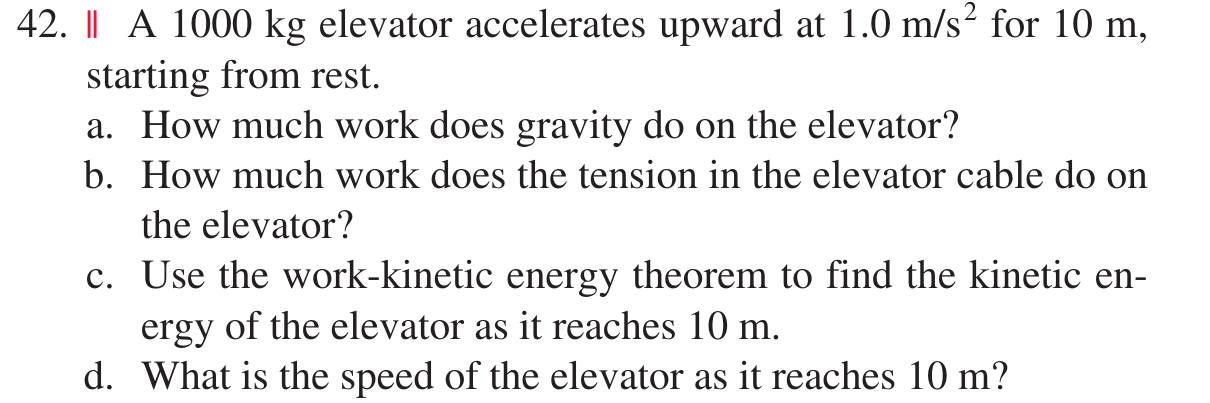
\includegraphics[width=0.7\textwidth]{elevator.png}
}


\frame{\frametitle{\textbf{Sample problems}}
  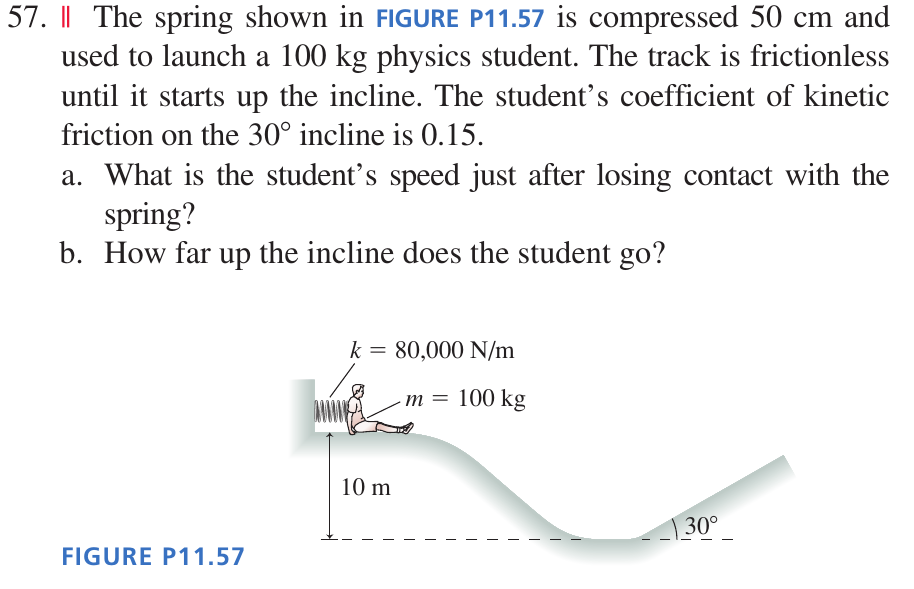
\includegraphics[width=0.7\textwidth]{student-on-spring.png}
}

\frame{\frametitle{\textbf{Sample problems}}
  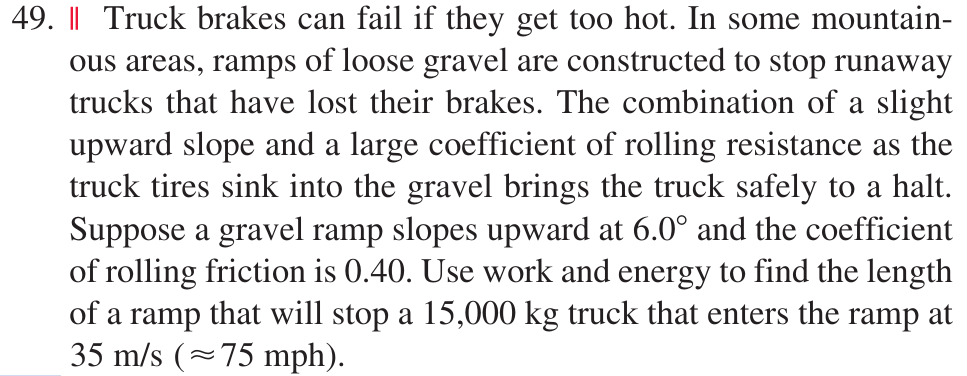
\includegraphics[width=0.7\textwidth]{runaway.png}
}





\end{document}
